\section{Personnages}
Les personnages avec un ‘ \textbf{*} ’ sont des Jokers, ils possèdent une fiche de perso jouable. 

\subsection{Reine de Ktath’Atn} \label{sec:ktath-atn-queen}
\begin{figure}[h!]
    \centering
    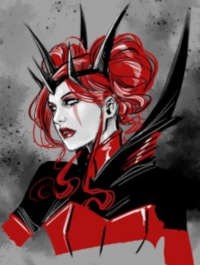
\includegraphics[height=250pt]{_img/pnjs/ktath-atn-queen.png}
\end{figure}
\subsubsection{Background}
Femme mystérieuse qui dirige la \textbf{Citadelle Hurlante} sur la planète Ktath’atn en l’an 0. Chaque année, elle organise une soirée durant laquelle elle reçoit de nombreux civils venus lui présenter des formes de vie organiques "intéressantes". Celui qui présente la forme de vie la plus intéressante se voit alors accorder un veux par la reine.
\newpage
\begin{paperbox}{Pouvoirs de la reine}
La reine, grace à sa compétence \textit{Symbiose Parfaite} possède des pouvoirs non basé sur la Force. Ces pouvoirs font d’elle un combattant redoutable malgrés son illusoire absence d’aptitudes au combat. Voici le fonctionnement et les effets de ces pouvoirs, jouez le comme l’Arcane \textit{Science \'Etrange} de \citetitle{savage-worlds} mais sans l’objet associé.
\bigbreak
\begin{rebelist}
    \item \textbf{Téléportation [3pt]}: Grâce à sa faculté de téléportation, la reine est capable de se déplacer instantanément d’un endroit à l’autre de la citadelle. Ce pouvoir compte pour le déplacement du round. Pour se téléporter vers un endroit qu’elle ne voit pas, la reine a un malus de \textbf{-2}. EN cas d’échec critique, un 1, la reine subit \textbf{2d6} de dommages.
    \item \textbf{Choc Psychique [2pt]}: La reine est capable d’émettre une sorte d’onde psychique qui va étourdir tous les enemies sur un rayon de 6m autour d’elle. En cas de succés, les victimes doivent réussir un jet de \textbf{Vig}ueur sinon elles se retrouvent secouées. En cas de Relance, le jet de \textbf{Vig}ueur subit un malus de \textbf{-2}.
    \item \textbf{\'Eclair [1-3pt]}: Le reine concentre sa psyché en une énergie tangible. Sous la forme d’un éclair qui foudroit ses enemis. Elle peut créer 1 à 3 éclair, chaque éclair coute un point de pouvoir supplémentaire. S’ils touchent chaque éclair fait \textbf{2d6}. La puissance peut être monté à \textbf{3d6} si la reine concentre trois éclairs en un seul point.
    \item \textbf{Dissipation [3pt]}: La reine est capable de contrer les pouvoirs de la Force. Elle peu dissiper un pouvoir en cours ou, si elle est en attente, contrer un pouvoir dont elle est la cible, le jet de \textit{Symbiose} vient donc contrer le jet de Force.
    \item \textbf{Augmentation [2pt]}: La reine peut augmenter l’un de ses Traits d’un dé, voire deux avec une Relance. L’augmentation dure 3 tours et demande \textbf{1pt} de pouvoir supplémentaire par tour.
\end{rebelist}
\end{paperbox}
\newpage

\begin{tikzpicture}[overlay, anchor=north]
    \node at (9,2) {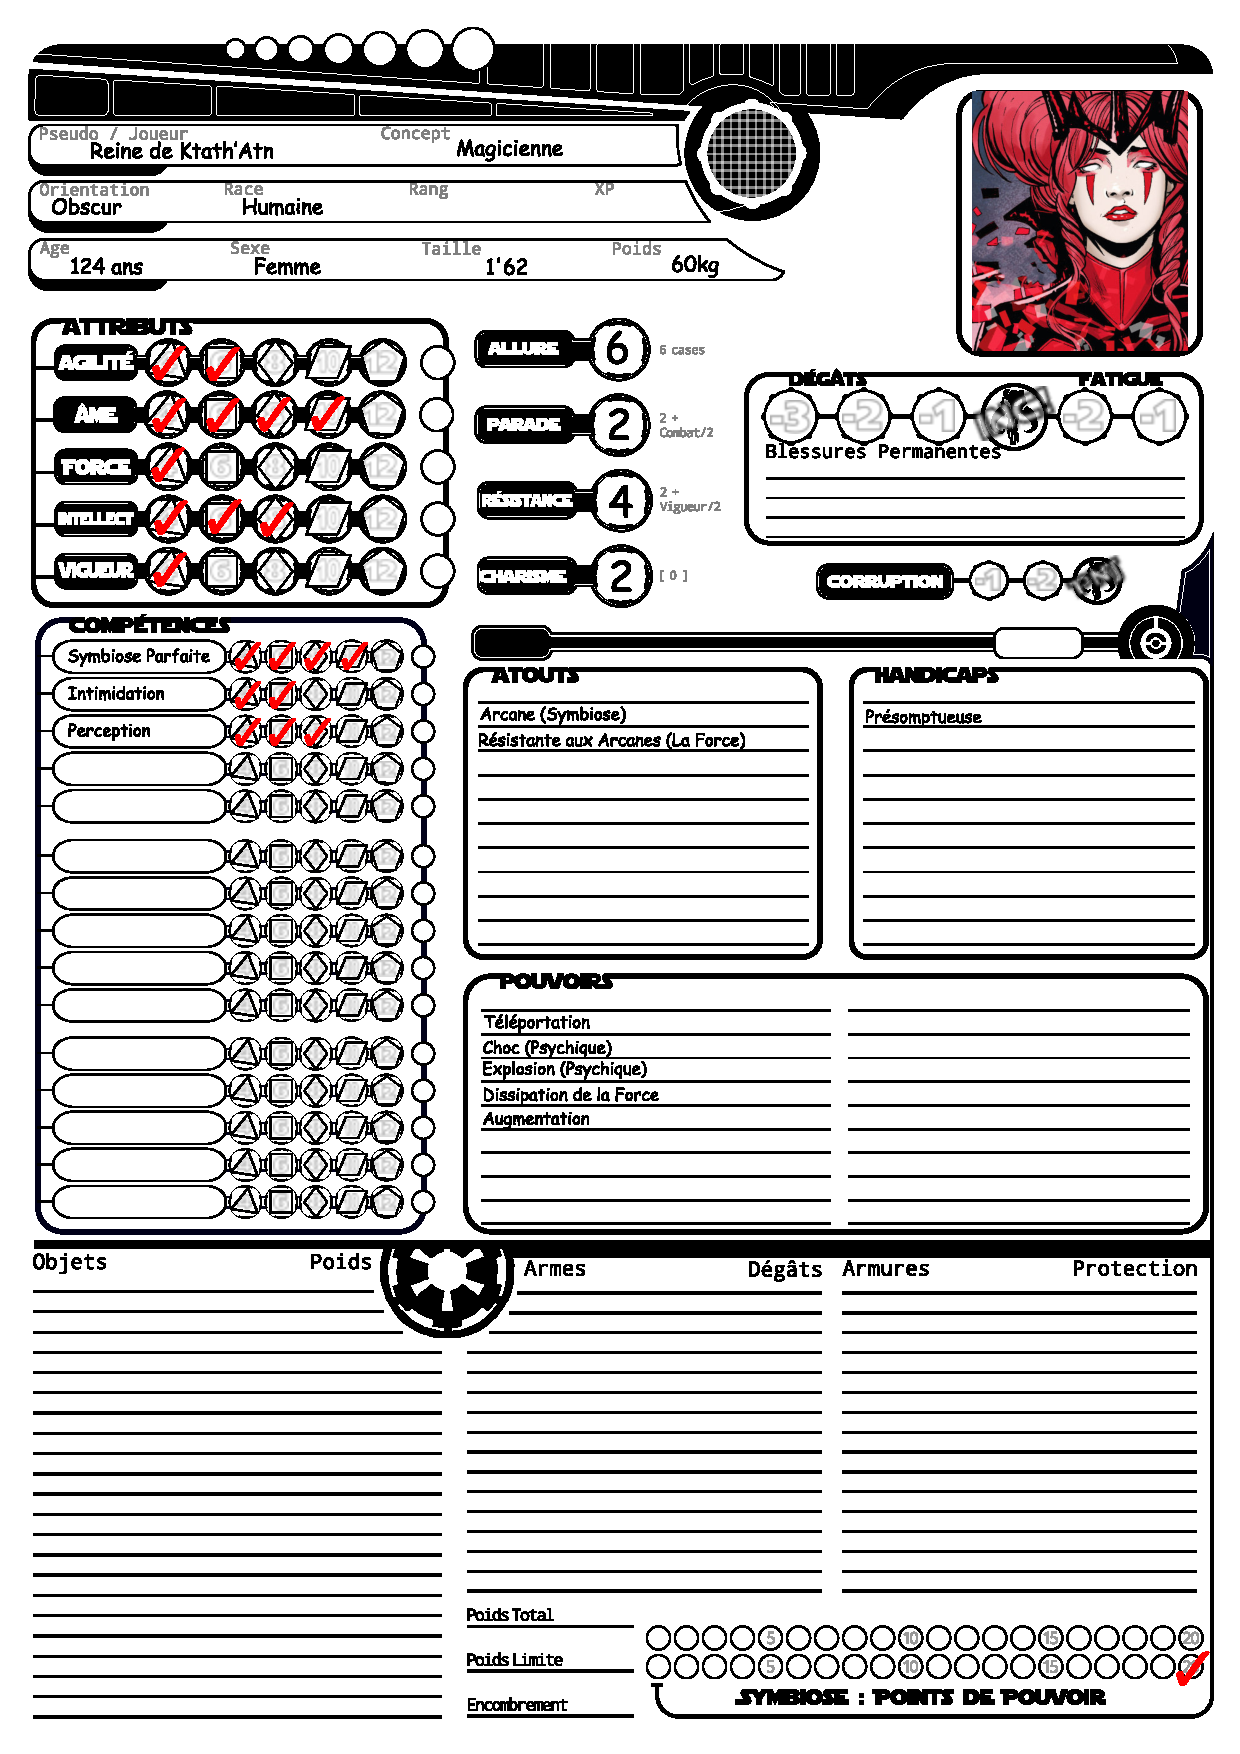
\includegraphics[height=0.99\paperheight]{_img/pnjs/fiche-ktath-atn-queen.pdf}};
\end{tikzpicture}

\clearpage

\subsection{Aphra} \label{sec:aphra}
\begin{figure}[h!]
    \centering
    
\includegraphics[height=250pt]{_img/pnjs/aphra.png}
\end{figure}
\subsubsection{Background}
Chelli Lona Aphra, nommée d’après sa défunte mère Lona Aphra, surnommée Boop par son père, et appelée Aphra par le reste du monde, était une archéologue et contrebandière. Elle travailla notamment pour Dark Vador après la destruction de l’Étoile de la Mort. Jeune femme séduisante au tempérament bien trempé, brune avec des électrotatouages sur le bras droit, elle sait ce qu’elle veut, admire les gens de pouvoir, et ne fait confiance qu’à elle-même pour survivre. 

\subsubsection{Traits}

\begin{itemtable}[ c c c c c ]
    \textbf{Agi} & \textbf{Int} & \textbf{\^Ame} & \textbf{For} & \textbf{Vig} \\
    d8           & d12          & d4             & d6           & d6           
\end{itemtable}
\begin{itemtable}[ l X ]
    \textbf{Allure}      & 6 \\
    \textbf{Compétences} & Connaissance(Archéologie) d10, Réparation d10, Tir d8 \\
    \textbf{Atouts}      & Bidouilleur, Voleur, Acolyte(Wookie)
\end{itemtable}

\subsubsection{Défense}
\begin{itemtable}[ c c ]
    \textbf{Parade}     & \textbf{Résistance} \\
    6                   & 5 
\end{itemtable}

\newpage

\subsection{Bombinax} \label{sec:bombinax}
\begin{figure}[h!]
    \centering
    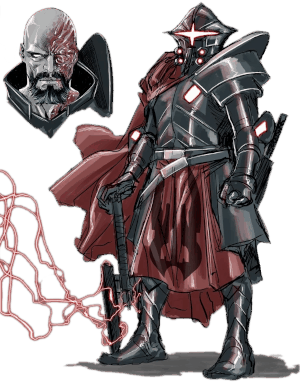
\includegraphics[height=250pt]{_img/pnjs/bombinax.png}
\end{figure}
\newpage

\subsection{Varroa} \label{sec:varroa}
\begin{figure}[h!]
    \centering
    
\includegraphics[height=250pt]{_img/pnjs/varroa.png}
\end{figure}

\newpage
\subsection{Vespinax} \label{sec:vespinax}
\begin{figure}[h!]
    \centering
    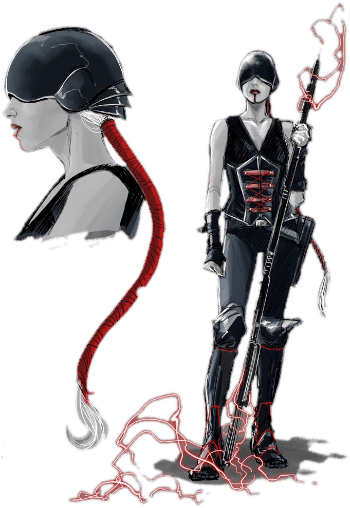
\includegraphics[height=250pt]{_img/pnjs/vespinax.png}
\end{figure}
